\documentclass[polish,a4paper]{article}
\usepackage[utf8]{inputenc}
\usepackage[T1]{fontenc}
%%\usepackage{polski}
\usepackage{amsmath}
\usepackage{amssymb,amsfonts,amsthm}
\usepackage{babel}
\usepackage{hyperref}
\usepackage{xcolor}
\usepackage{graphicx} 
\usepackage{caption}
\usepackage{subcaption}
\usepackage{listings}
\usepackage{anysize}
%%\usepackage{tabto}

\graphicspath{ {img/} }
\title{Arduino – elementy pomiarowe (SW lab02)}
\author{Olga Gerlich 148088, Kamil Kałużny 148121 grupa I1.2}
\marginsize{2.5cm}{2.5cm}{0cm}{3cm}

\definecolor{codegreen}{rgb}{0,0.6,0}
\definecolor{codegray}{rgb}{0.5,0.5,0.5}
\definecolor{codepurple}{rgb}{0.58,0,0.82}
\definecolor{backcolour}{rgb}{0.95,0.95,0.92}

\lstdefinestyle{mystyle}{
	backgroundcolor=\color{backcolour},   
	commentstyle=\color{codegreen},
	keywordstyle=\color{magenta},
	numberstyle=\tiny\color{codegray},
	stringstyle=\color{codepurple},
	basicstyle=\ttfamily\footnotesize,
	breakatwhitespace=false,         
	breaklines=true,                 
	captionpos=b,                    
	keepspaces=true,                 
	numbers=left,                    
	numbersep=5pt,                  
	showspaces=false,                
	showstringspaces=false,
	showtabs=false,                  
	tabsize=2
}

\lstset{style=mystyle}

\begin{document}
	\maketitle
	\section{Termometr (DS18B20) – One wire}
	\begin{figure}[h!]
		\begin{center}
			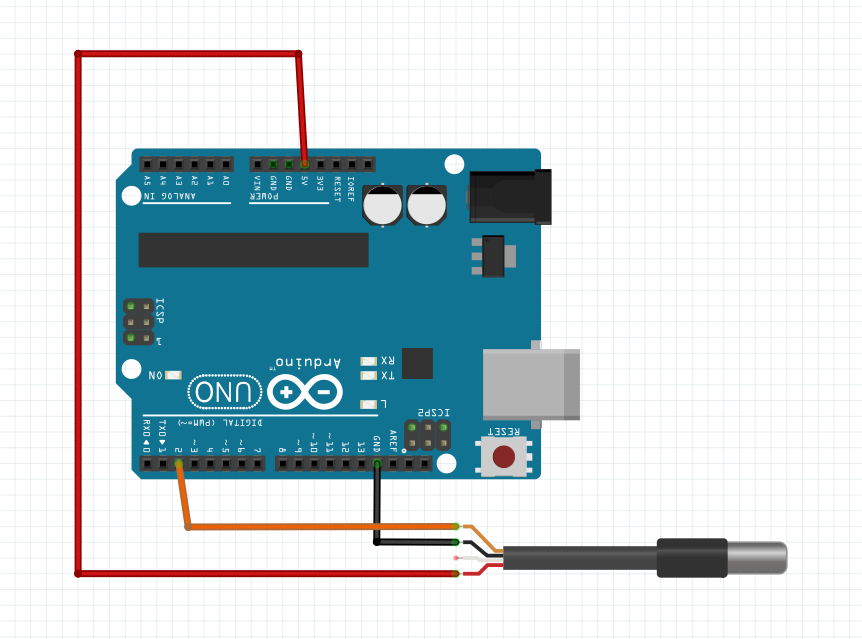
\includegraphics[scale=0.42]{01_temp_sensor.png}
			\caption*{Schemat podłączenia termometru do Arduino}
		\end{center}
	\end{figure}
	\begin{figure}[h!]
		\begin{lstlisting}[language=C++, basicstyle=\tiny]
			#include <OneWire.h>
			const byte ONEWIRE_PIN = 2;
			OneWire onewire(ONEWIRE_PIN);
			DS18B20 sensors(&onewire);
			
			void setup(){
				while(!Serial);
				Serial.begin(9600);
			}
			
			void loop(){
				byte address[8];
				onewire.reset_search();
				while(onewire.search(address))
				{
					if (address[0] != 0x28)
					continue;
					
					if (OneWire::crc8(address, 7) != address[7]){
						Serial.println(F("Bledny adres, sprawdz polaczenia"));
						break;
					}
					
					for (byte i=0; i<8; i++){
						Serial.print(F("0x"));
						Serial.print(address[i], HEX);
						
						if (i < 7)
						Serial.print(F(", "));
					}
					Serial.println();
				}
				while(1);
			}
			// wypisany na Serial Monitor adres:
			// 0x28, 0xFF, 0xBC, 0x88, 0x90, 0x17, 0x5, 0x76
		\end{lstlisting}
		\caption*{Kod użyty do wyznaczenia adresu czujnika}
	\end{figure}
	
	\begin{figure}[h!]
		\begin{lstlisting}[language=C++, basicstyle=\tiny]
			#include <OneWire.h>
			#include <DS18B20.h>
			#include <SPI.h>
			#include <MFRC522.h>
			
			#define ONEWIRE_PIN 2
			
			// Adres czujnika
			byte address[8] = {0x28, 0xFF, 0xBC, 0x88, 0x90, 0x17, 0x5, 0x76};
			
			OneWire onewire(ONEWIRE_PIN);
			
			int sort_desc(const void *cmp1, const void *cmp2){
				int a = *((int *)cmp1);
				int b = *((int *)cmp2);
				return a > b ? -1 : (a < b ? 1 : 0);
			}
			
			void setup() {
				while(!Serial);
				Serial.begin(9600);
				SPI.begin();      // Initiate  SPI bus
				sensors.begin();
				sensors.request(address);
			}
			
			void loop() {
				float vec[20];
				if (sensors.available())
				{
					for (int i = 0; i < 18; i++) {
						vec[i] = sensors.readTemperature(address);
					}
					qsort(vec, 18, sizeof(float), sort_desc);
					
					float sum = 0;
					for (int i = 1; i < 17; i++) {
						sum += vec[i];
					}
					sum /= 16;
					
					Serial.print(sum);
					Serial.println(F(" 'C"));
					sensors.request(address);
				}
			}
		\end{lstlisting}
		\caption*{Kod użyty do wyznaczenia średniej temperatury}
	\end{figure}
	\subsection{Opis działania OneWire}
	OneWire jest interfejsem komunikacyjnym. Nazwa wynika z tego, że do komunikacji między urządzeniami wyposażonymi w ten interfejs wystarczy jedna linia transmisyjna (nie licząc masy). OneWire ma strukturę Master-Slave, co oznacza, że urządzenie nadrzędne (Master) wysyła komendy do urządzeń podrzędnych (Slave), których może być wiele. W celu odróżnienia slave od siebie, nadaje się im unikatowe 64-bitowe numery seryjne. 
	
	Komunikacja na linii danych przebiega w dwie strony, z tego powodu dołącza się do magistrali bufory trójstanowe lub bramki z otwartym drenem, w celu utrzymania porządku wysyłania danych. 
	
	Master rozpoczyna transmisję danych poprzez wystawienie impulsu reset. To powoduje zresetowanie wszystkich podłączonych urządzeń podrzędnych, które następnie wysyłają impuls obecności na linię danych. Od tego momentu, master może przesyłać sekwencje bitów do slave'ów. Urządzenie podrzędne wykona określone akcje, tylko w przypadku gdy dane polecenie dotyczy tego urządzenia. Master odczytuje dane z urządzeń slave.
	
	\newpage
	\section{RFID}
	\begin{figure}[h!]
		\begin{center}
			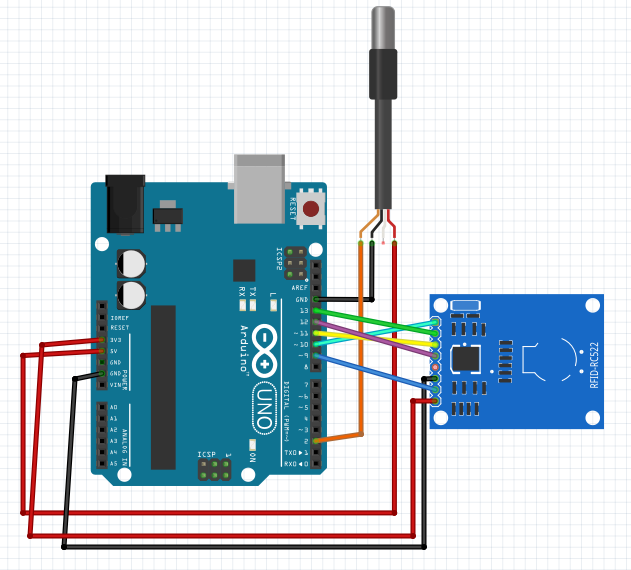
\includegraphics[scale=0.4]{02_rfid_reader.png}
			\caption*{Schemat podłączenia RFID do Arduino}
		\end{center}
		\begin{lstlisting}[language=C++, basicstyle=\tiny]
			#include <OneWire.h>
			#include <DS18B20.h>
			#include <SPI.h>
			#include <MFRC522.h>
			#define SS_PIN 10
			#define RST_PIN 9
			MFRC522 mfrc522(SS_PIN, RST_PIN);   // Create MFRC522 instance.
			#define ONEWIRE_PIN 2
			
			// Adres czujnika
			byte address[8] = {0x28, 0xFF, 0xBC, 0x88, 0x90, 0x17, 0x5, 0x76};
			OneWire onewire(ONEWIRE_PIN);
			DS18B20 sensors(&onewire);
			
			int sort_desc(const void *cmp1, const void *cmp2){
				int a = *((int *)cmp1);
				int b = *((int *)cmp2);
				return a > b ? -1 : (a < b ? 1 : 0);
			}
			
			void setup() {
				while(!Serial);
				Serial.begin(9600);
				SPI.begin();      // Initiate  SPI bus
				mfrc522.PCD_Init();   // Initiate MFRC522
				sensors.begin();
				sensors.request(address);
			}
			
			void loop() {
				float vec[20];
				if (sensors.available()){
					for (int i = 0; i < 18; i++) {
						vec[i] = sensors.readTemperature(address);
					}
					qsort(vec, 18, sizeof(float), sort_desc);
					
					float sum = 0;
					for (int i = 1; i < 17; i++) {
						sum += vec[i];
					}
					sum /= 16;
					
					if ( ! mfrc522.PICC_IsNewCardPresent()) return;
					if ( ! mfrc522.PICC_ReadCardSerial()) return;
					
					String content= "";
					byte letter;
					for (byte i = 0; i < mfrc522.uid.size; i++){
						content.concat(String(mfrc522.uid.uidByte[i] < 0x10 ? " 0" : " "));
						content.concat(String(mfrc522.uid.uidByte[i], HEX));
					}
					// adresy odczytane dzieki powyzszej petli:
					// C4 F7 2E D0 // brelok
					// 6D 3D AC 75 // karta
					content.toUpperCase();
					if (content.substring(1) == "BD 31 15 2B"){
						Serial.print(sum);
						Serial.println(F(" 'C"));
					}
					else{
						Serial.println("Brak dostepu");
					}
					sensors.request(address);
				}
			}
		\end{lstlisting}
		\caption*{Kod źródłowy wyświetlający temperature po przyłożeniu karty do modułu RFID}
	\end{figure}
	\newpage
	\subsection{Opis działania SPI}
	SPI (Serial Peripheral Interface) to interfejs komunikacyjny pozwalający na komunikację full-duplex, czyli można jednocześnie wysyłać i odbierać dane. SPI jest również interfejsem synchronicznym - jeden z przewodów przesyła sygnał zegarowy, który synchronizuje wszystkie urządzenia podrzędne. Prędkość transmisji dostosowywana jest do najwolniejszego ze stosowanych układów. 
	
	Tak samo jak w interfejsie OneWire, SPI też ma strukturę typu Master-Slave. Również w tym przypadku, możliwe jest połączenie kilku układów slave, dołącza się bufor trójstanowy oraz tylko master może rozpocząć transmisję. Dodatkowo, master może generować sygnał zegarowy.
	
	\begin{figure}[h!]
		\begin{center}
			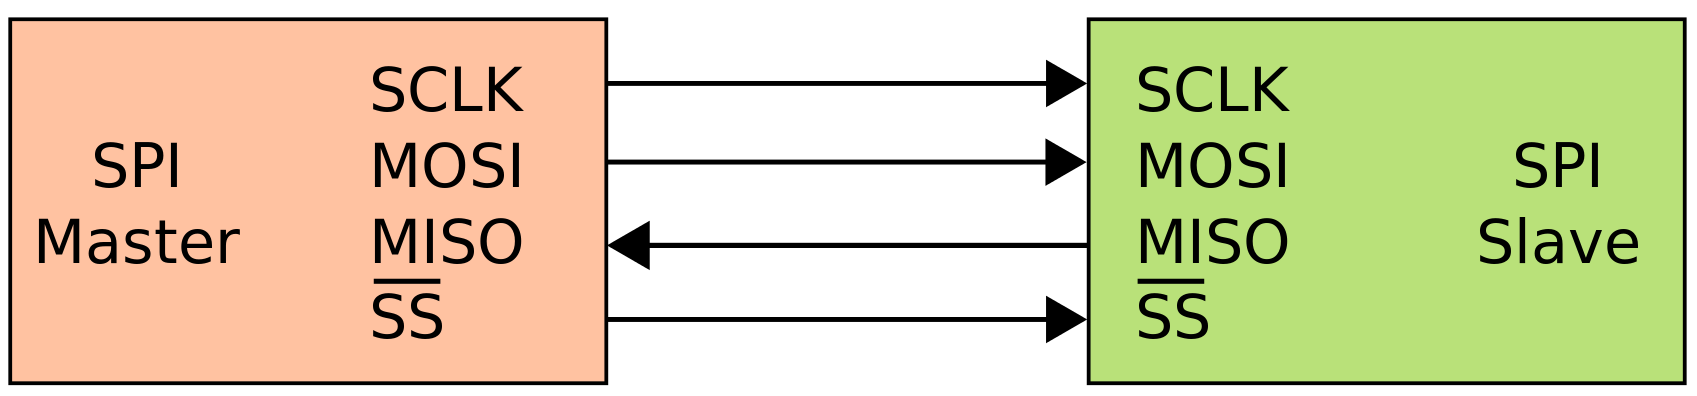
\includegraphics[scale=0.2]{SPI.png}
			\caption*{Przykładowa konfiguracja układów master oraz slave w systemie.}
		\end{center}
	\end{figure}
	
	Magistrala SPI składa się najczęściej z czterech linii. Są to:
	\begin{itemize}
		\item MOSI (master out, slave in) – linia łącząca wyjście danych z mastera i wejścia slave’ów
		\item MISO (master in, slave out) – linia łącząca wyjście danych slave i wejście mastera
		\item SCLK (serial clock) – sygnał zegarowy, synchronizujący układy na magistrali
		\item CS (chip select), SS (slave select) – pozwala na wybranie układu, który będzie przeprowadzał transmisję
	\end{itemize}
	
	Aby rozpocząć transmisję, master musi wysłać sygnał zegarowy i wybrać układ, ściągając do masy odpowiednią linię CS. Linie MISO i MOSI tworzą pierścień, przez co układy slave i master mogą jednocześnie wysyłać dane do siebie nawzajem. Dane są synchronicznie przenoszone na linię MOSI i czytane z linii MISO. 
	
	\newpage
	\section*{Źródła}
	\begin{enumerate}
		\item \href{https://fritzing.org/}{Fritzing}
		\item \href{https://github.com/miguelbalboa/rfid/blob/master/doc/fritzing/RFID-RC522-v2.fzpz}{RFID}
		\href{https://github.com/adafruit/Fritzing-Library/blob/master/parts/DS18B20%201-Wire%20Temperature%20Sensor%20Probe%20Cable.fzpz}{DS18B20}
		\item Materiały podane przez prowadzącego na platformie ekursy.
		\item \href{https://randomnerdtutorials.com}{randomnerdtutorials}
		\item \href{https://www.youtube.com/watch?v=TCMo1yASYvw}{1-Wire RS Elektronika}
		\item \href{http://extronic.pl/content/60-kurs-xmega-interfejs-spi}{Interfejs SPI - Extronic}
		\item \href{https://www.elektroda.pl/rtvforum/topic3551692.html}{Wprowadzenie do interfejsu SPI - elektroda} 
	\end{enumerate}
	\begingroup
	\hypersetup{hidelinks}
	\tableofcontents
	\endgroup
\end{document}
